\documentclass[18pt,a4paper]{article}
\usepackage[ngerman]{babel}
\usepackage[T1]{fontenc}

\usepackage[utf8]{inputenc}
\usepackage{setspace}
\usepackage{amsmath}
\usepackage{amsfonts}

\usepackage{fancyhdr}
\usepackage{graphicx}
%\usepackage[yyyymmdd]{datetime}
%\renewcommand{\dateseparator}{}
%\usepackage{datetime2}

\pagestyle{fancy} %eigener Seitenstil
\fancyhf{} %alle Kopf- und Fußzeilenfelder bereinigen
\fancyhead[L]{Reihen} %Kopfzeile links
\fancyhead[C]{Fabian Pfaff} %zentrierte Kopfzeile
\fancyhead[R]{\today} %Kopfzeile rechts
\fancyfoot[L]{Reihen}
\fancyfoot[C]{\thepage} %Seitennummer
\fancyfoot[R]{\today}
\renewcommand{\footrulewidth}{0.4pt} %untere Trennlinie

\begin{document}
\section*{Aufgabe 9}
Bestimmen Sie die ersten drei Summanden, welche nicht null sind, der Maclaurin-Reihe von $f(x) = tan(x)$.\\
Die Mclaurin-Reihe lautet:\\
\begin{equation*}
\sum_{i=0}^{n}\frac{f^{(i)}(0)}{i!}\cdot x^i = \frac{f^{(0)}(0)}{0!}\cdot x^0+\frac{f^{(1)}(0)}{1!}\cdot x^1+\frac{f^{(2)}(0)}{2!}\cdot x^2 \dots
\end{equation*}
\begin{align*}
tan(x) &= \frac{sin(x)}{cos(x)}\\
\intertext{\flushleft Nach der Quotientenregel ergibt sich die erste Ableitung}\\
tan'(x) &= \frac{cos^2(x)+sin^2(x)}{cos^2(x)}\\
\intertext{Jetzt gibt es zwei Möglichkeiten zu kürzen. Entweder wird $cos^2(x)+sin^2(x) = 1$ gesetzt oder man löst den Bruch auf. Je nach Aufgabe erleichtert die eine oder andere Darstellung. Hier wird folgender Ausdruck verwendet}\\
tan'(x) &= \frac{cos^2(x)}{cos^2(x)} + \frac{sin^2(x)}{cos^2(x)}\\
tan'(x) &= 1 + tan^2(x)
\end{align*}
Die restlichen Ableitungen lauten:\\
\begin{align*}
f^{(1)}(x) &=  1 + tan^2(x)  \qquad  &f^{(1)}(0) &= 1 \\
f^{(2)}(x) &=  2\cdot tan(x) + tan^3(x)  \qquad  &f^{(2)}(0) &= 0 \\
f^{(3)}(x) &=  2 + 8\cdot tan^2(x) + 6\cdot tan^4(x) \qquad  &f^{(3)}(0) &= 2 \\
f^{(4)}(x) &=  16\cdot tan(x) + 40 \cdot tan^3(x) + 24 \cdot tan^5(x )\qquad  &f^{(4)}(0) &= 0 \\
f^{(5)}(x) &=  16 + 136 \cdot tan^2(x) + 240\cdot tan^4(x) + 120\cdot tan^6(x)  \qquad  &f^{(5)}(0) &= 16 \\
\end{align*}
Setzen wir das nun in die Definition der Mclaurin Reihe erhält man folgenden Ausdruck:\\
\begin{equation*}
tan(x) \approx 0 + x + 0 +\frac{2}{3!}x^3 + 0 + \frac{16}{5!}x^5 = x + \frac{1}{3}x^3 + \frac{2}{15}x^5
\end{equation*}
\newpage
\begin{figure}[t]
	\centering
	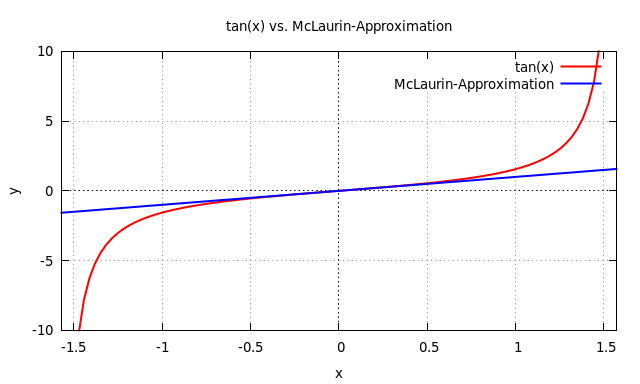
\includegraphics[width=1\linewidth]{plots/output}
	\caption{Plot der Tangensfunktion (rot) und der McLaurin-Approximation (blau) im Bereich von -$\pi/2$ bis $\pi/2$}
	\label{fig:output}
\end{figure}

\null
\vfill

\end{document}